% Name: Union–find forest
% Description: Two disjoint sets stored as trees whose nodes point to their parents, each root pointing to itself, with the parent array that stores the same forest below.
% Tags: union-find, disjoint set, forest, data structures

\usetikzlibrary{arrows.meta}

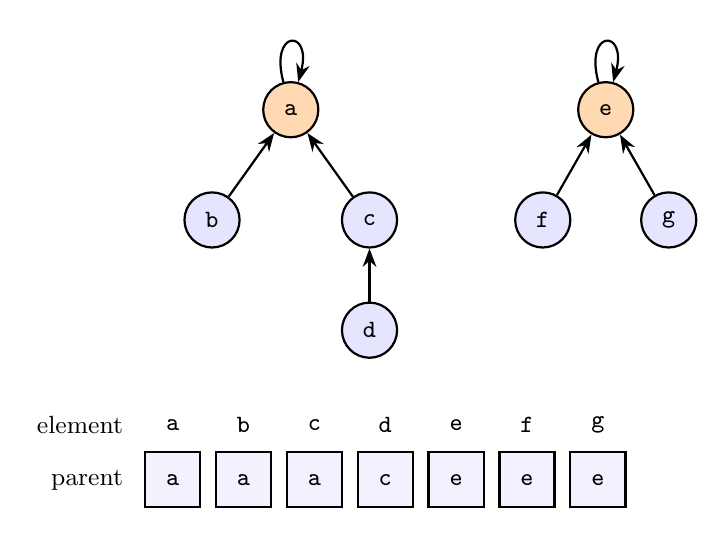
\begin{tikzpicture}[>={Stealth}, thick,
    v/.style={circle, draw, fill=blue!10, minimum size=7mm, font=\small\ttfamily},
    root/.style={v, fill=orange!30}]
  \node[root] (a) at (1.5,3) {a};
  \node[v] (b) at (0.5,1.6) {b};
  \node[v] (c) at (2.5,1.6) {c};
  \node[v] (d) at (2.5,0.2) {d};
  \node[root] (e) at (5.5,3) {e};
  \node[v] (f) at (4.7,1.6) {f};
  \node[v] (g) at (6.3,1.6) {g};
  \foreach \u/\p in {b/a, c/a, d/c, f/e, g/e} \draw[->] (\u) -- (\p);
  \foreach \r in {a, e} \draw[->] (\r) edge[loop above, min distance=7mm] (\r);
  % The same forest as an array: parent[x] for each element x
  \foreach \x/\p [count=\i from 0] in {a/a, b/a, c/a, d/c, e/e, f/e, g/e} {
    \node[font=\small\ttfamily] at (0.9*\i,-1) {\x};
    \node[draw, minimum size=7mm, font=\small\ttfamily, fill=blue!5] at (0.9*\i,-1.7) {\p};
  }
  \node[anchor=east, font=\small] at (-0.5,-1) {element};
  \node[anchor=east, font=\small] at (-0.5,-1.7) {parent};
\end{tikzpicture}
